\section{CSS}

Per lo sviluppo di un sito web il ramo della presentazione risulta molto importante. Abbiamo cercato di creare un layout fluido, semplice ed intuitivo per tutti considerando che ogni persona e' un potenziale cliente come gia' mezionato nel capitolo di analizi utenza.
Il sito e' diviso fondamentalmente in 6 sezioni:
\begin{itemize}
	\item \textbf{Header} sempre nella parte superiore della pagina contiene il Titolo del centro sportivo e \textbf{Path} che risulta utile quando si accede alla pagina per la registrazione e durante la prenotazione di un campo poiche' sono 2 pagine di 'secondo livello'
	\item	\textbf{Navigation} consiste nel menu' con tutti i link utili per la navigazione nel sito
	\item \textbf{Content} sempre al centro della pagina consiste nel contenuto del sito, contiene tutte le informazioni utili, la pagina di registrazione e tutti i form per la prenotazione dei campi da gioco.
	\item \textbf{Login} presente in ogni pagina contiene un piccolo form per effettuare l'accesso al sito o un link per andare alla registrazione per un nuovo utente.
	\item \textbf{News} e' un piccolo riquadro con le varie news inserite dall'amministratore
	\item \textbf{footer} posto sempre nella parte inferiore del sito contiene le immagini delle varie validazioni.
\end{itemize}

\subsection{Differenze su diversi terminali}

Abbiamo utilizzato le \textbf{mediaquery} per ottenere diversi layouts su vari terminali.
qui sotto riportiamo delle immagini per mostrare alcune di queste differenze:

\begin{figure}
	{\centering 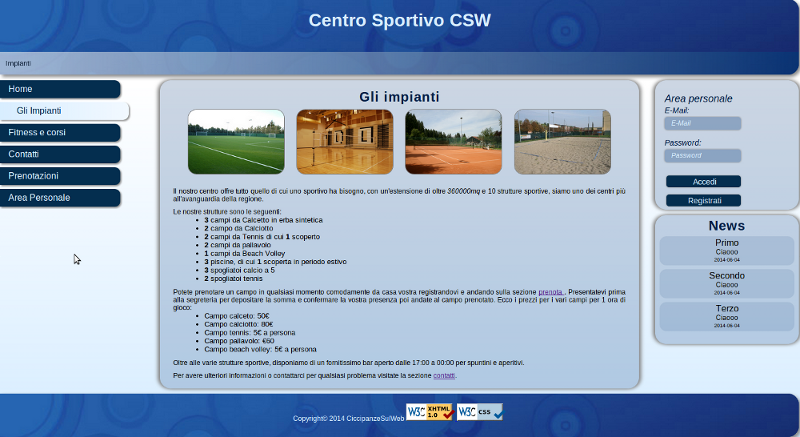
\includegraphics[height=0.3\textwidth]{images/normal.png} 
	\caption{a) style}}
\end{figure}
\begin{figure}
	{\centering 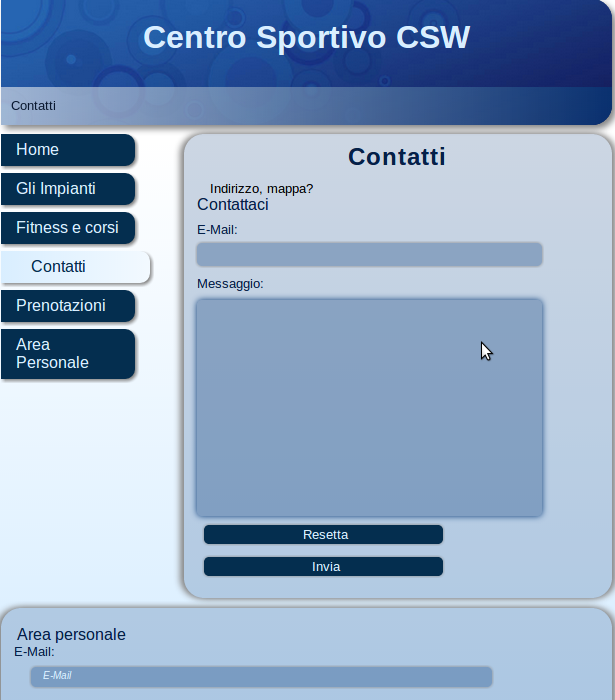
\includegraphics[height=0.3\textwidth]{images/tablet.png} 
	\caption{b) tablet} }
\end{figure}
\begin{figure}
	{\centering 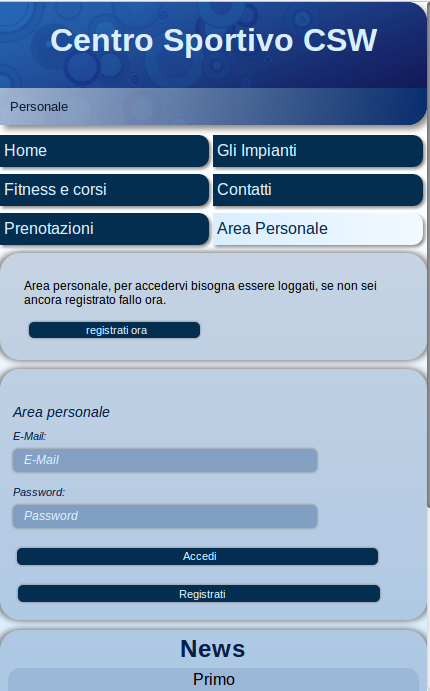
\includegraphics[height=0.3\textwidth]{images/mobile.png} 
	\caption{c) mobile}}
\end{figure}

Su dispositivi con risoluzioni alte abbiamo deciso di usare un layout a 3 colonne mentre come possiamo notare su dispositivi con media risoluzione come tablet abbiamo deciso di spostare semplicemente la parte Login e News sotto per lasciare piu' spazio al contenuto essendo di maggiore importanza.
Su dispositivi mobile abbiamo messo tutto in colonna.

\subsection{Compatibilita'}

Nello sviluppo della parte di presentazioni abbiamo usato qualche regola CSS non compatibile con tutti i browsers o non con tutte le versioni.
Per un maggior supporto abbiamo utilizzato diversi \textbf{vendor prefix} quali \textbf{-moz},\textbf{-o},\textbf{-webkit}
Per la compatibilita' di queste regole abbiamo effettuato delle ricerche online e basandoci su alcuni siti come \textbf{http://caniuse.com/}.
possiamo ad esempio vedere la compatibilita' di 'Transition' nei vari browser cosi': \newline \newline
 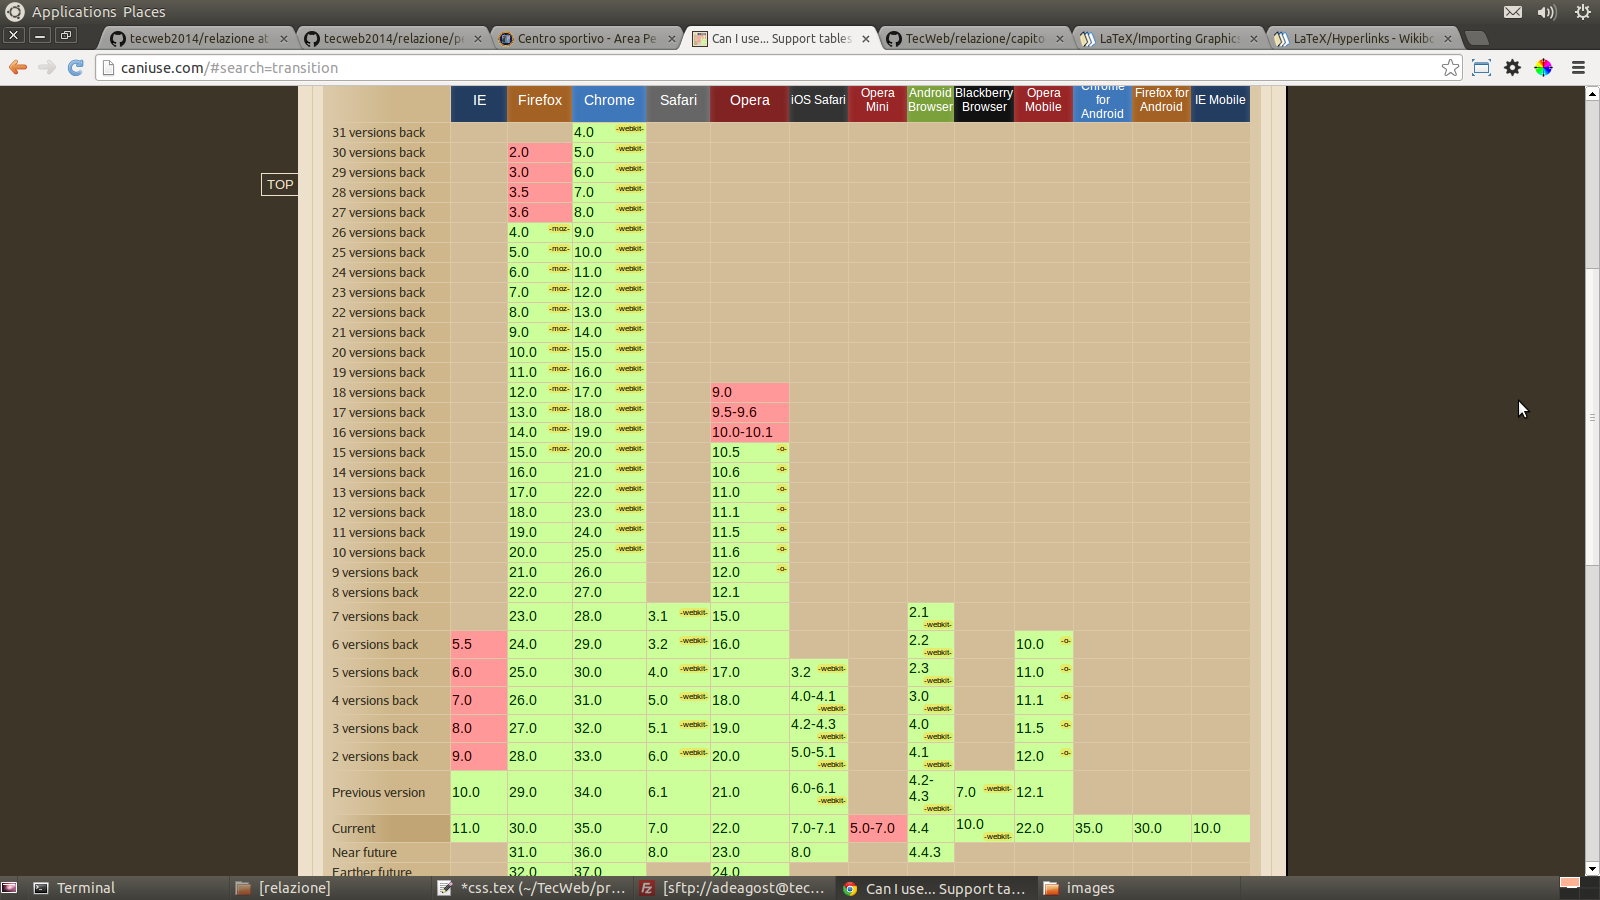
\includegraphics[width=0.7\textwidth]{images/caniuse1.png} \newline
Altre regole sono:
\begin{itemize}
	\item rgba che ha un 90\% di compatibilita' globale
	\item border-radius usato per arrotondare header, footer e varie immagini e' supportato da tutti i browser eccetto opera mini, da IE9 e da firefox con prefisso -moz fino alla versione 3.6 anche senza successivamente.
	\item box-shadow supportato da tutte le versione recenti di tutti i browser eccetto opera mini, mentre per alcune versioni vecchie servono prefissi come -webkit per chrome fino a versione 9
\end{itemize}

In ogni caso anche con versioni che non supportano queste regole css troviamo sempre un fallback elegante, il sito risulta essere meno accattivante tuttavia il funzionamento e la dispozione generale del sito non cambiano rimanendo cosi' accettabile con ogni browser.\newline
Per i test di compatibilita' sono stati effettuati con tutti i browser che sono presenti nel laboratorio Paolotti che sono i seguenti:
\begin{itemize}
	\item chrome versione 34.0 nessun problema
	\item chromium versione 34.0 nessun problema
	\item firefox versione 28.0 nessun problema
	\item konqueror versione 4.5 con questo browser la navigazione e' pressoche' impossibile, si riscontrano molti problemi quali il non supporto a nessuna delle regole css precedentemente elencate, non rispetta il ridimensionamento delle immagini, alcuni link addirittura risultano non funzionanti.
Tuttavia dopo alcune ricerche in internet abbiamo deciso deliberatamente di tralasciarlo viste le bassissime percentuali di utilizzo nel mondo.
	\item Opera versione 12.16 salvo qualche differenza come il colore dei placeholder tutto risulta funzionare normalmente.
	\item Internet Explorer versione ? tutto funziona correttamente apparte i placeholder che hanno un carattere piu' "marcato" su questo browser 
	\item Safari versione ? Transition risulta essere lento e con questo browser le immagini vengono ridimensionate in base alla grandezza della finestra senza rispettare la regola css
\end{itemize}

Abbiamo anche effettuato test con Chrome disabilitando tutti gli stili o eliminando tutte le immagini e la navigazione sul sito non risultava compromessa.
